\chapter{Headlands}
\label{ch:headlands}

The experiment of Chapter~\ref{ch:measuring} showed the problem every mowing
pattern must solve first: parallel passes need room to turn at their ends,
and that room, a band along the border called the \emph{headland}, must
itself be mowed. This chapter builds the headland passes: closed paths that
follow the border of the lawn, and of each hole, at a fixed distance, and
that the mower can drive without leaving the lawn.

\section{Offsetting the lawn}

\begin{definition}{Offset region}{offset}
  The \emph{offset} of the lawn $\Omega$ by a distance $c \ge 0$ is the set of
  points at distance at least $c$ from the outside of $\Omega$ (the region
  beyond the border and the holes):
  \[
    \Omega_c = \{\, p \in \Omega : \operatorname{dist}(p, \R^2 \setminus
    \Omega) \ge c \,\}.
  \]
  In mathematical morphology it is the \emph{erosion} of $\Omega$ by the disc
  of radius $c$: the set of centres of the discs of radius $c$ that fit in
  $\Omega$.
\end{definition}

When $\Omega$ is a polygon with holes, $\Omega_c$ is bounded by segments
parallel to the edges of $\Omega$ at the distance $c$, and by arcs of radius
$c$ around the reflex corners of $\Omega$ (where the border juts into the
lawn). The code uses the geometry library Shapely, whose \code{buffer(-c)}
computes $\Omega_c$, and replaces the arcs by sharp corners (``mitred
joins''): a corner then stays a single vertex, which the planner treats once.
As $c$ grows, the holes grow, and the region can pinch and split
(Figure~\ref{fig:offsets}).

\begin{figure}[ht]
  \centering
  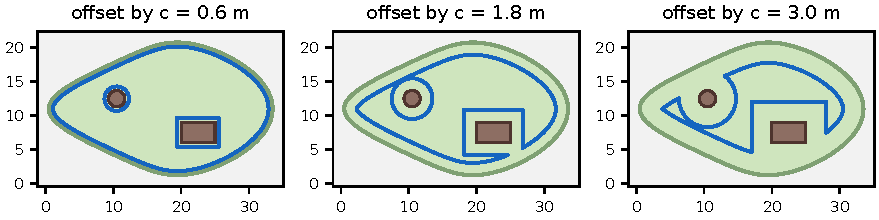
\includegraphics[width=\textwidth]{figures/offsets}
  \caption{The garden of Figure~\ref{fig:lawns} offset by three distances
    (blue: the boundary of $\Omega_c$). At \SI{0.6}{\metre} the offset
    follows the border and goes round the two holes; at \SI{1.8}{\metre} the
    flower bed's ring has merged with the border's, through the narrow gap
    between them; at \SI{3}{\metre} the region is about to split in two.}
  \label{fig:offsets}
\end{figure}

The $k$-th headland pass follows the boundary of $\Omega_{c_k}$, with
\[
  c_k = c_1 + (k - 1)\,s,
\]
where $s$ is the spacing between passes (the cutting width minus a small
overlap, $s = 0.97 - 0.05 = \SI{0.92}{\metre}$). Each boundary curve is
walked with the lawn on its left: counter-clockwise along the border,
clockwise around a hole. What remains is to choose $c_1$, and to turn these
curves into paths the mower can drive.

\section{How close to the border?}

Driving straight along the border, the middle of the rear axle must stay at
least $h + m$ from it, where $h$ is the half-width of the mower
(\SI{0.515}{\metre}, the deck housing) and $m$ a safety margin
(\SI{5}{\centi\metre}). In a turn, the mower needs more room.

\begin{proposition}{Swing-out}{swingout}
  On a left arc of radius $R$, a point $(a, b)$ of the mower (mower frame)
  stays at the distance $\sqrt{a^2 + (R - b)^2}$ from the centre of rotation
  $C = (0, R)$. On the right of the mower, the outline therefore reaches
  \[
    e(R) = \max_{(a, b) \in \text{outline}} \sqrt{a^2 + (R - b)^2}
      \;-\; (R + h)
  \]
  farther from $C$ than it does in a straight line. For a front corner
  $(a, -b)$, the excess $\sqrt{a^2 + (R + b)^2} - (R + b)$ is reached when
  the heading has turned by $\psi^* = \arctan\bigl(a / (R + b)\bigr)$.
\end{proposition}

\begin{proof}
  By Proposition~\ref{prop:icr}, every point of the mower moves on a circle
  about $C$, and by Pythagoras the point $(a, b)$ is at the distance
  $\sqrt{a^2 + (R - b)^2}$ from $C = (0, R)$. Along the rear axle, the right
  side of the mower is at the lateral position $-h$, at the distance $R + h$
  from $C$; this is how far the mower reaches on that side when it only
  translates. During the turn each point keeps its distance to $C$ while
  its direction from $C$ rotates with the mower, so in any fixed direction
  it reaches out to that distance, when the vector from $C$ to the point
  points that way. Hence the excess $e(R)$.

  For the front corner $(a, -b)$, the vector from $C$ is $(a, -(R + b))$; it
  makes the angle $\arctan\bigl(a/(R + b)\bigr)$ with the rear axle
  direction $(0, -1)$, which is the direction of the right side. The mower
  turns left, so after it has turned by that angle, the vector points along
  the original rear axle direction: the corner is then farthest out on the
  right, at $\sqrt{a^2 + (R + b)^2}$ from $C$.
\end{proof}

\begin{figure}[ht]
  \centering
  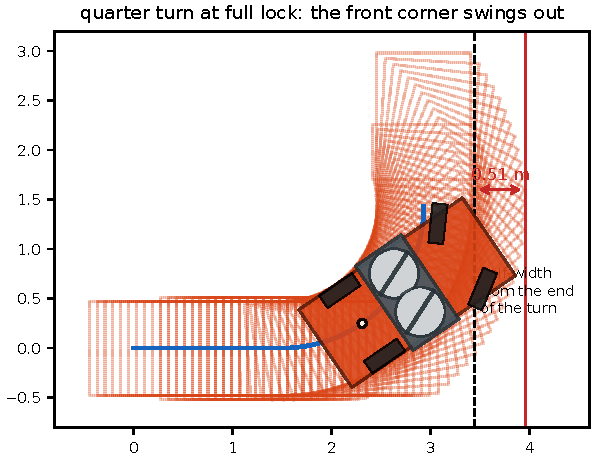
\includegraphics[width=0.62\textwidth]{figures/swing}
  \caption{A quarter turn at full lock to the left after a straight start:
    the outline of the mower at successive positions (red). At the end of
    the turn, heading north, the right side of the mower would be at the
    dashed line if it had only translated; during the turn its front corner
    went \SI{0.51}{\metre} beyond it.}
  \label{fig:swing}
\end{figure}

\begin{example}{Swing-out of the default mower}{swingnum}
  The front corner of the body is at $(a, -b) = (1.55, -0.475)$, and $h =
  0.515$. At full lock ($R = \SI{1.43}{\metre}$):
  \begin{align*}
    e &= \sqrt{1.55^2 + (1.43 + 0.475)^2} - (1.43 + 0.515) \\
      &= \sqrt{2.4025 + 3.6290} - 1.945 = 2.4559 - 1.945 = \SI{0.511}{\metre},
  \end{align*}
  reached after $\psi^* = \arctan(1.55/1.905) = 39.1°$. On wider arcs the
  swing-out shrinks: \SI{0.30}{\metre} at $R = \SI{2.86}{\metre}$,
  \SI{0.15}{\metre} at \SI{5.72}{\metre}, \SI{0.06}{\metre} at
  \SI{11.4}{\metre}.
\end{example}

\begin{inwords}
  A car's front corner swings out in a turn, so following a fence round a
  bend needs more clearance than driving straight along it, and a tight bend
  needs much more. The same effect appears when the mower steers back onto a
  line parallel to a wall: during the last arc its nose leads, and sticks
  out by up to $e$ of that arc. This is why the outermost headland pass
  cannot simply run at $h + m$ from the border.
\end{inwords}

The code therefore uses a first clearance
\[
  c_1 = h + m + \varepsilon,
\]
with the smallest extra slack $\varepsilon$ (by steps of
\SI{5}{\centi\metre}) for which every corner of the first ring has a
collision-free path (Section~\ref{sec:corners}). On the rectangle and the
L-shaped lawn, $\varepsilon = \SI{0.05}{\metre}$ and $c_1 =
\SI{0.615}{\metre}$; the garden, with its sharp tip, needs
$\varepsilon = \SI{0.50}{\metre}$ and $c_1 = \SI{1.065}{\metre}$. Along the
border, a strip of width $c_1 - w/2$ is out of reach of the blades
(\SI{0.13}{\metre} on the rectangle): on a real lawn, the job of a string
trimmer. A clearance that varies along the border, larger only near tight
bends, would reduce it on the garden; it is a refinement left for later.

\section{Following a curved border}

A curved border is a polygon with many vertices, each turning by a few
degrees. The mower cannot follow the sharp angles of the polygon, but it can
follow circular arcs tangent to its edges.

\begin{proposition}{Fillet}{fillet}
  At a vertex where the path turns by the angle $\varphi$, an arc of radius
  $\rho$ tangent to both edges starts and ends at the distance
  $t = \rho\tan(|\varphi|/2)$ from the vertex. Since the arcs of two
  consecutive vertices must not overlap, $t$ may not exceed half of either
  adjacent edge, so the largest possible radius is
  \[
    \rho_{\max} = \frac{\min(\ell_{\mathrm{prev}}, \ell_{\mathrm{next}})}
      {2\tan(|\varphi|/2)} .
  \]
\end{proposition}

\begin{proof}
  The centre of an arc tangent to both edges lies on the bisector of the
  angle between them, at the distance $\rho$ from each edge. The two
  tangent points and the vertex form, with the centre, two right triangles
  whose angle at the centre is $|\varphi|/2$ (the arc turns by $|\varphi|$),
  so the distance from the vertex to each tangent point is
  $\rho\tan(|\varphi|/2)$.
\end{proof}

The planner gives each vertex of the offset polygon the radius
$\rho_{\max}$: on a finely sampled curve, consecutive arcs then meet and
reproduce the curve. A vertex is a \emph{bend}, followed by its arc, if it
turns by at most $20°$ and $\rho_{\max} \ge \Rmin$; otherwise it is a
\emph{corner}. On a bend that turns left, the swing-out of
Proposition~\ref{prop:swingout} may exceed the slack: the planner moves the
vertices of such bends inwards by the missing clearance, plus
\SI{5}{\centi\metre}, taking for each vertex the largest shortfall within
\SI{1.5}{\metre} along the ring, so that the pushed ring stays smooth.

\section{Corners}
\label{sec:corners}

At a corner, the planner looks for the best of two manoeuvres, in this
order.

\paragraph{Shift and turn.}
Move inwards by a distance $\delta$ with an S-curve, turn with an arc of
radius $\rho \ge \Rmin$ tangent to the two shifted edges, and shift back.
An S-curve made of two opposite arcs of radius $R_s$, each turning by
$\alpha$, moves the mower sideways without changing its heading:

\begin{proposition}{S-curve}{scurve}
  Two arcs of radius $R_s$, the first turning left by $\alpha$ and the
  second right by $\alpha$, shift the mower sideways by
  $\delta = 2R_s(1 - \cos\alpha)$ and forward by $2R_s\sin\alpha$, with the
  same final heading. For a given shift,
  $\alpha = \arccos\bigl(1 - \delta/(2R_s)\bigr)$.
\end{proposition}

\begin{proof}
  By Proposition~\ref{prop:arc} with $\theta_0 = 0$, the first arc ends at
  $\bigl(R_s\sin\alpha,\; R_s(1 - \cos\alpha)\bigr)$ with heading $\alpha$.
  The second arc, of curvature $-1/R_s$, starts at heading $\alpha$ and ends
  at heading $0$; by the same proposition it moves by
  $\bigl(-R_s(\sin 0 - \sin\alpha),\; R_s(\cos 0 - \cos\alpha)\bigr) =
  \bigl(R_s\sin\alpha,\; R_s(1 - \cos\alpha)\bigr)$. Adding both gives the
  result.
\end{proof}

The search tries $\delta$ from $0$ to \SI{1.5}{\metre} by steps of
\SI{0.1}{\metre}, then $\rho \in \{\Rmin, \Rmin + 0.5, \Rmin + 1, \Rmin +
2\}$ and $R_s \in \{2\Rmin, 4\Rmin, 8\Rmin\}$ (a wider S-curve swings out
less), and keeps the first combination whose path keeps the whole mower on
the lawn and fits in the edges around the corner.

\paragraph{Manoeuvre with reverse.}
If no shifted turn fits, the planner stops at a distance $b$ before the
corner on the incoming edge and joins the outgoing edge at $b$ after it with
the fastest Reeds--Shepp path that stays on the lawn
(Chapter~\ref{ch:paths}); $b$ grows from $0$ by steps of
\SI{0.2}{\metre}.

\paragraph{No manoeuvre.}
Where the offset region pinches (Figure~\ref{fig:offsets}, middle), the ring
can have a near-hairpin corner that nothing can follow. The ring is then cut
there: it becomes an open path, which the mower drives in whichever
direction is easier to reach. Two corners closer than \SI{2}{\metre} are
first merged into one, at the meeting point of the edges before and after
them, since no manoeuvre fits between them.

\begin{figure}[ht]
  \centering
  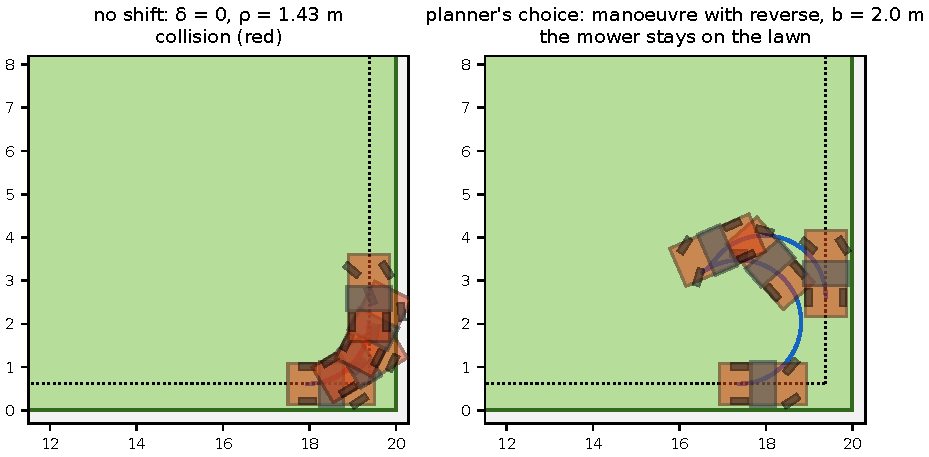
\includegraphics[width=\textwidth]{figures/corner}
  \caption{The bottom-right corner of the rectangle for the first headland
    pass ($c_1 = \SI{0.615}{\metre}$; dotted: the offset lines), with the
    mower drawn at four moments. Left: a plain arc at full lock; the front
    corner swings out of the lawn (red: poses in collision with the lawn
    shrunk by the safety margin). Right: what the planner does: a manoeuvre
    with a reverse leg (red dashed), started \SI{2}{\metre} before the
    corner.}
  \label{fig:corner}
\end{figure}

\section{How many headland passes?}

The main passes end where the mower must turn. A turn into the next pass
sticks out by $a_{\mathrm{turn}}$ beyond the rear axle at the end of the pass
(\SI{2.46}{\metre} for the fastest three-point turn of
Section~\ref{sec:nextpass}, including the front of the mower), so a pass
must end at $a_{\mathrm{turn}} + m$ from the border. Its blades cut up to
$d + r$ ahead of the rear axle, so a depth of $a_{\mathrm{turn}} + m - (d
+ r)$ along the border is left for the headland. The $k$-th headland pass
cuts up to $c_1 + (k - 1)s + w/2$ from the border.

\begin{proposition}{Number of headland passes}{headlandcount}
  The headland passes cut the whole depth left by the main passes if their
  number $n$ satisfies
  \[
    c_1 + (n - 1)\,s + \frac w2 \;\ge\; a_{\mathrm{turn}} + m - (d + r),
  \]
  that is, for the smallest such $n$,
  \[
    n = 1 + \Bigl\lceil \frac{a_{\mathrm{turn}} + m - (d + r) - c_1
      - w/2}{s} \Bigr\rceil .
  \]
\end{proposition}

\begin{example}{Two passes}{twopasses}
  With $a_{\mathrm{turn}} = 2.456$, $m = 0.05$, $d + r = 0.80$,
  $c_1 = 0.615$, $w/2 = 0.485$ and $s = 0.92$:
  \[
    n = 1 + \Bigl\lceil \frac{2.456 + 0.05 - 0.80 - 0.615 - 0.485}{0.92}
      \Bigr\rceil = 1 + \lceil 0.659 \rceil = 2 .
  \]
\end{example}

This count assumes that the border is perpendicular to the passes. Where it
is oblique, the turn needs more room, and Chapter~\ref{ch:swaths} shortens
the passes until every turn is collision-free.

\section{Joining the passes}

The planner drives the rings one after the other, outermost first. From the
end of one ring it tries several entry points on the next (closest first),
and keeps the fastest Reeds--Shepp connection that stays on the lawn, with
the blades off. Where obstacles block every direct connection, it searches
a path around them (the search of Chapter~\ref{ch:order}).

\begin{figure}[ht]
  \centering
  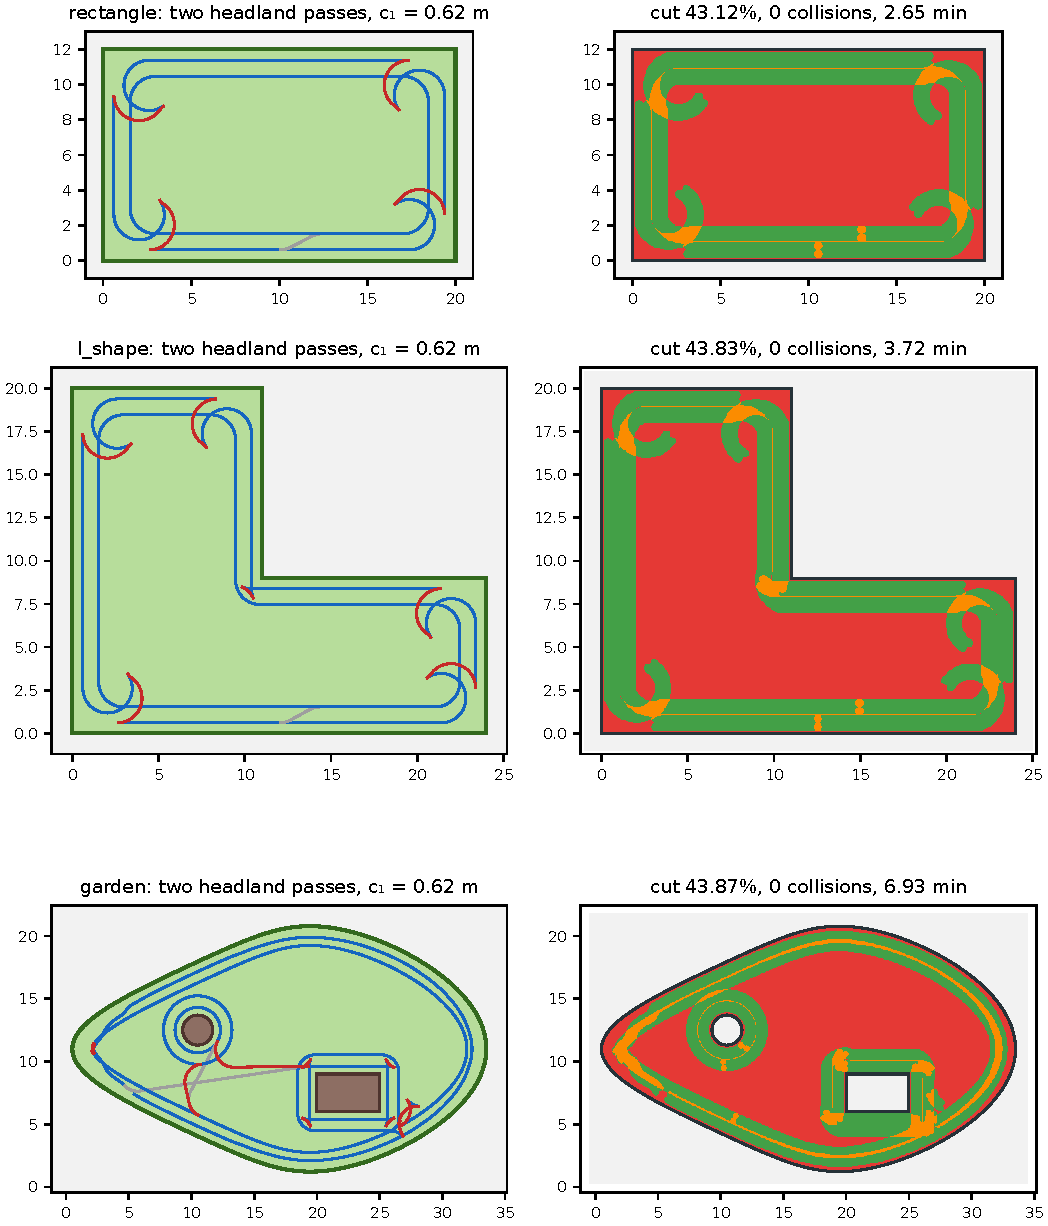
\includegraphics[width=\textwidth]{figures/headlands}
  \caption{Two headland passes on the three example lawns (left: the path of
    the rear axle, blue forward, red dashed reverse, grey with the blades
    off; right: the grass cut, green once, orange twice, red not yet). The
    interior is left for the main passes of the next chapter; the corners of
    the first ring on the rectangle and the L-shape are three-point
    manoeuvres, those of the second ring simple arcs.}
  \label{fig:headlands}
\end{figure}

\begin{center}
\begin{tabular}{@{}lrrrr@{}}
  \toprule
  lawn & $c_1$ & cut & collisions & time \\
  \midrule
  rectangle & \SI{0.615}{\metre} & 43.1\% & 0 & \SI{2.65}{\minute} \\
  L-shape & \SI{0.615}{\metre} & 43.8\% & 0 & \SI{3.72}{\minute} \\
  garden & \SI{1.065}{\metre} & 42.4\% & 0 & \SI{7.13}{\minute} \\
  \bottomrule
\end{tabular}
\end{center}

\begin{incode}
  \code{mowersim/planning/headland.py}: \code{swing\_out}
  (Proposition~\ref{prop:swingout}), \code{classify} (bends and corners,
  Proposition~\ref{prop:fillet}), \code{push\_tight\_bends},
  \code{shift\_arcs} (Proposition~\ref{prop:scurve}), \code{corner\_path},
  \code{solve\_corner\_shift}, \code{solve\_corner}, \code{build\_ring},
  \code{plan\_headland}, \code{headland\_passes\_needed}
  (Proposition~\ref{prop:headlandcount}) and \code{link\_rings}.
  \code{mowersim/planning/common.py}: the collision checker \code{Checker}
  (footprint outline and interior points against the lawn shrunk by the
  margin) and \code{connect}, the fastest collision-free Reeds--Shepp
  candidate.
\end{incode}
